\subsection{Atividades profundas} \label{sec:deep_activities}

% Definição de atividades profundas

Quando uma empresa modela seu processo de negócios em um BPM, é possível que existam muitos passos para completá-lo. Cada passo ou etapa no processo é chamado de atividade e, quando existem muitas atividades em sequência, chamamos de atividades profundas dentro de um processo.

Atividades profundas são aquelas que, a partir do início do fluxo de trabalhos, exigem um grande número de atividades intermediarias até que elas fiquem disponíveis, sendo necessário executar cada atividade anterior para alcançá-la.

% Problema em grandes workflows

Workflows complexos tendem a ter uma profundidade grande, que torna difícil a busca e a inserção de novos dados por usuários que o utilizam. Grandes workflows também podem ter múltiplos usuários em passos diferentes dentro do workflow, tendo diferentes objetivos de execução.

As atividades profundas surgem frequentemente quando um ambientes de negócios envolve muitos processos complexos, como na indústria de manufatura, setor de serviços financeiros ou em empresas com cadeias de suprimentos complexas. Essas atividades podem ajudar a garantir que todos os processos sejam executados de maneira consistente e eficiente, e que os objetivos sejam alcançados de forma efetiva, mas aumentam a profundidade do workflow consideravelmente, como podemos ver no workflow complexo representado na figura~\ref{fig:centrareEstrutura}.

\begin{figure}
    \centering
    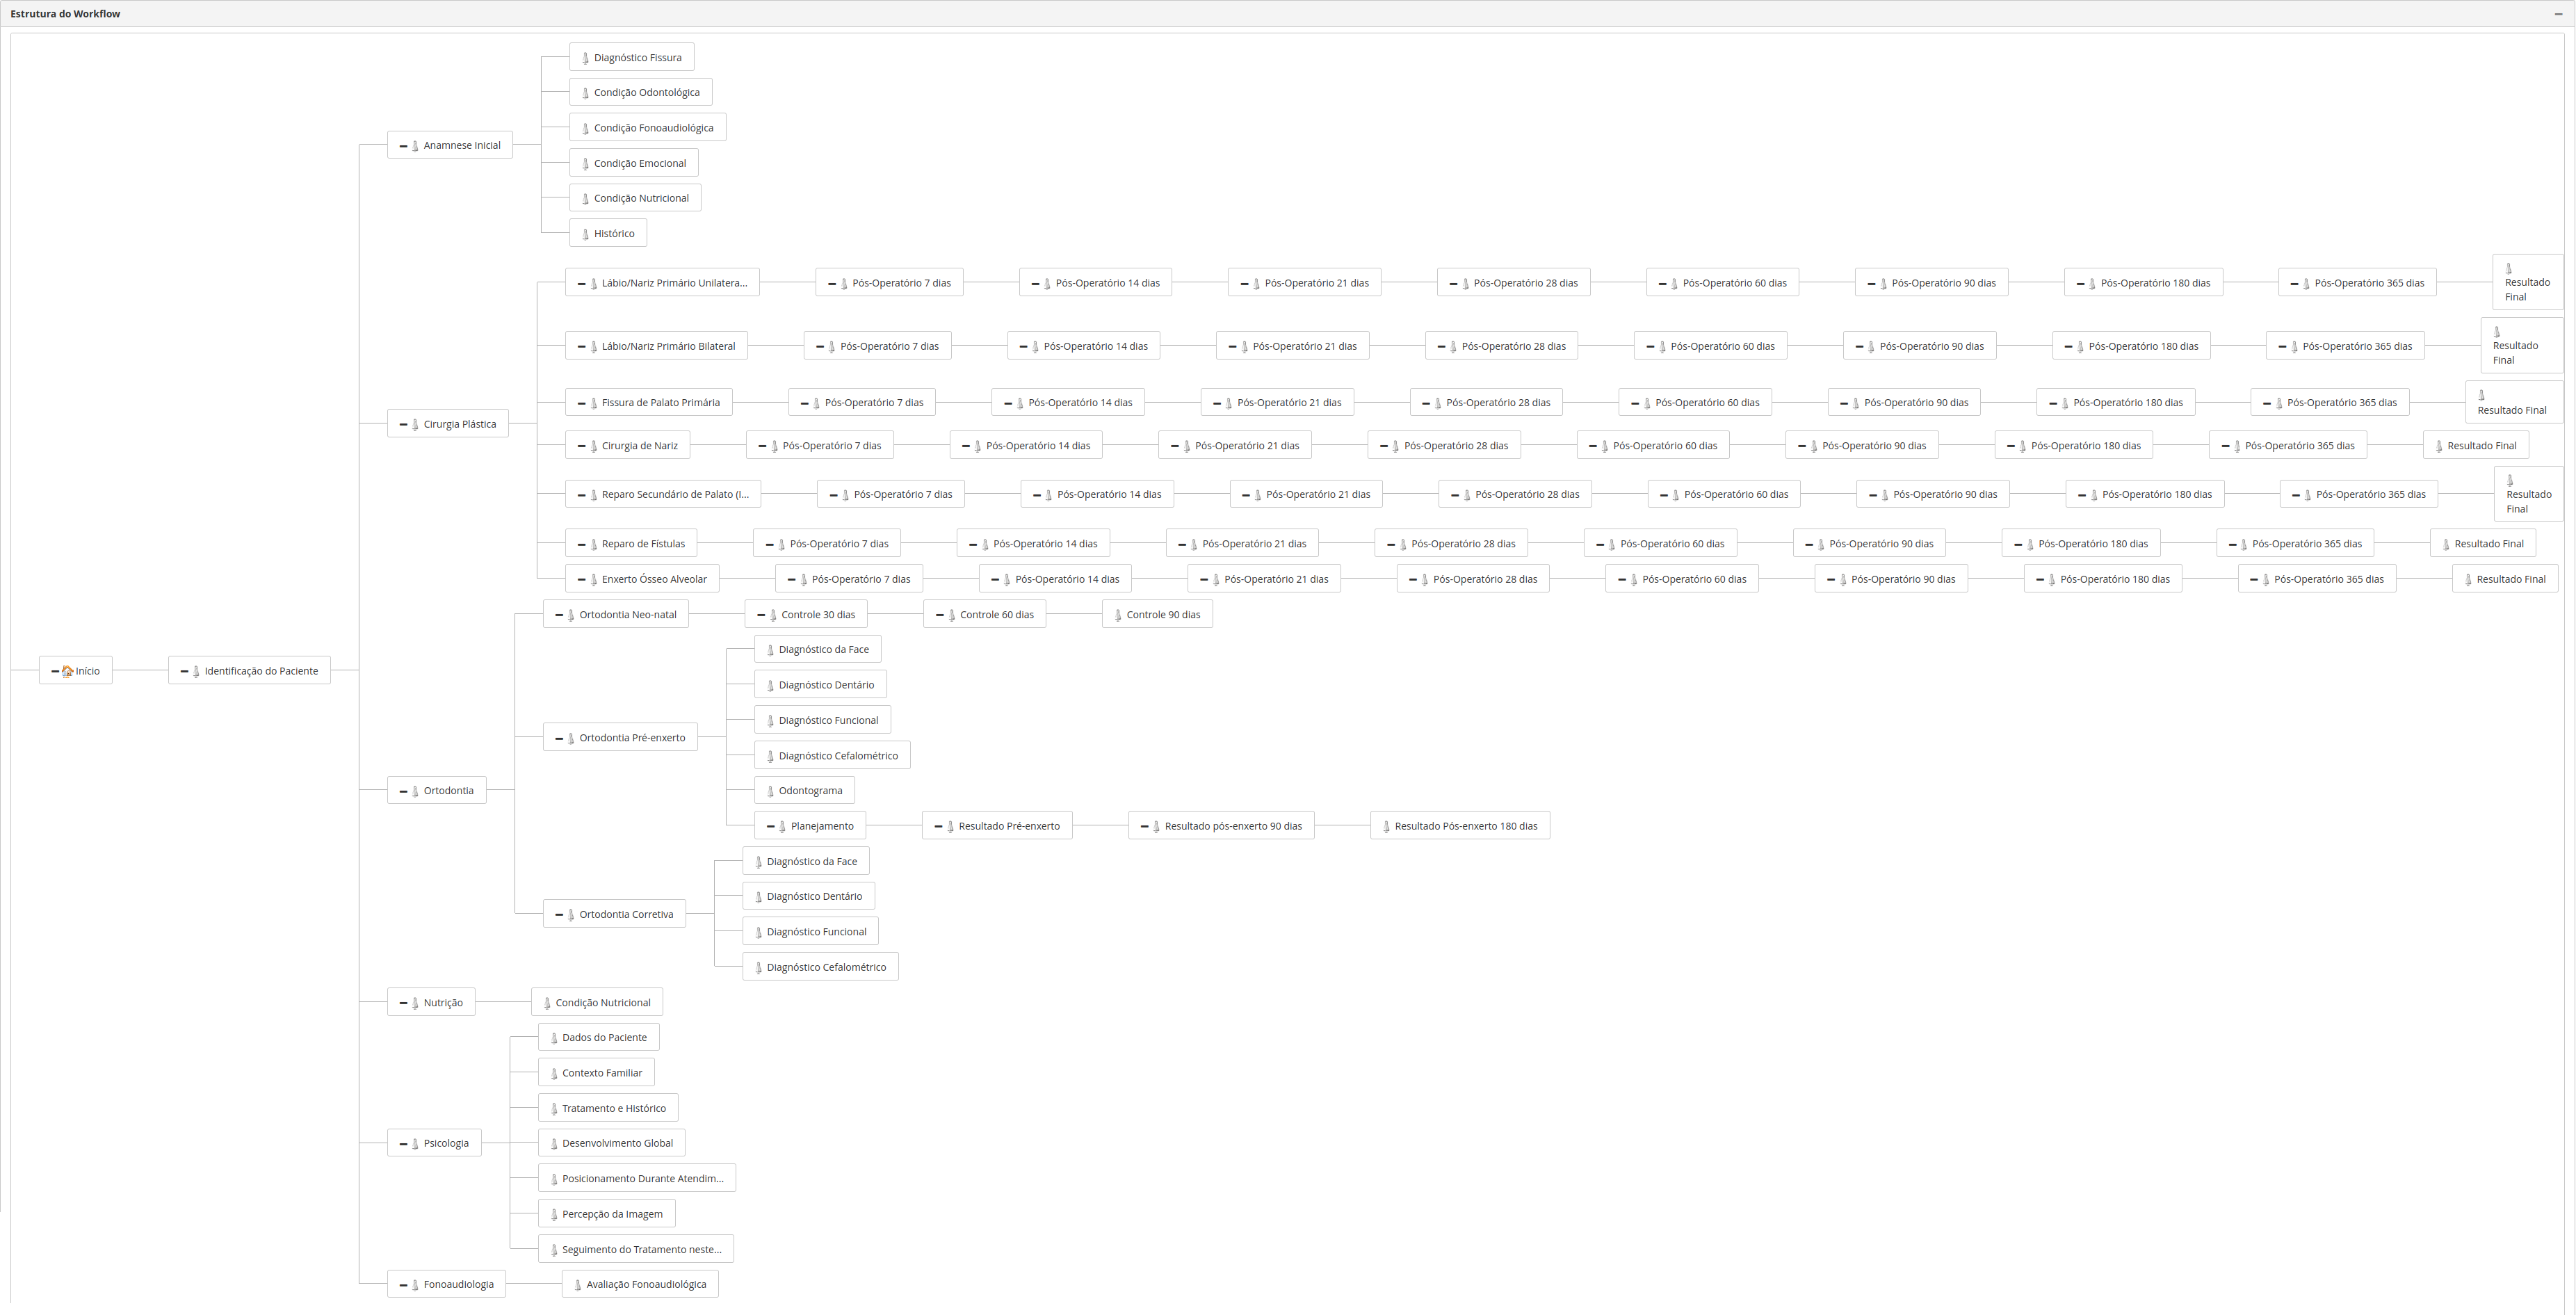
\includegraphics[width=1\textwidth]{imgs/CENTRARE/estrutura.png}
    \caption{Estrutura do workflow CENTRARE. Podemos verificar a quantidade de atividades em cada retângulo da estrutura em árvore, tendo um profundidade máxima de 12 atividades.}
    \label{fig:centrareEstrutura}
\end{figure}

O workflow apresentado na figura é o CENTRARE, que é um fluxo de trabalho para o Centro de Tratamento e Reabilitação de Fissura Labiopalatal e Deformidade Craniofacial do hospital da baleia, em Belo Horizonte.

Nele, é feito o acompanhamento de pacientes desde o nascimento até a adolescência por múltiplos médicos de diferentes áreas da saúde como odontologia, cirurgia plástica e psicologia. Este fluxo de trabalho é utilizado para o tratamento de lábios leporinos em crianças recém nascidas, com acompanhamento completo pós cirúrgico, familiar e nutricional.

% Porque isso é um problema

Este workflow é muito profundo e tem informações de anos acumuladas em um mesmo sistema. Essas atividades profundas podem virar um problema quando implementadas em um LIMS: Encontrar informações de maneira rápida e concisa pode não ser possível a depender das possibilidades de personalização de interface do LIMS, diminuindo a eficiência do trabalho dos funcionários que utilizam o software.

% Como isso se relaciona com Big Data

% Isso tem relação com a crescendo busca pela automatização de digitalização dos dados. Existem hoje informações sendo enviadas automaticamente para um sistema de coleta de dados por smart devices, como relógios ou ``smart bands'' que coletam dados de diversos tipos como dados cardiológicos, saturação de oxigênio, exercícios feitos pelo usuário, e isso aumenta a necessidade de softwares que coletam e armazenam dados com segurança.

% Este tipo de informações, por exemplo, pode ser utilizado em um sistema de telemedicina para coletar dados dos seus pacientes automaticamente, mandando notificações para o médico responsável pelo paciente caso algum dado precise de sua atenção.

A agregação, tratamento e disponibilização destes dados tanto para os usuários que o utilizam quanto para a empresa que os coletam é de grande importância para o desenvolvimento de soluções em aplicativos para saúde de usuários e também disponibilização de informações relacionadas com o estilo de vida das pessoas.

% Como isso se relaciona com a utilização com o médico

A necessidade de uma interface intuitiva, rápida e eficaz para os usuários chave de um LIMS é de muita importância para sua implementação também ajuda na implantação de um sistema LIMS por diminuir o atrito da adoção do software na organização, já que existe uma grande resistência na adoção de novas tecnologias, especialmente se estiverem acostumados a trabalhar com processos manuais ou sistemas legados~\cite{2018CommonAstrix}.

Essa resistência pode existir por alguns motivos como a complexidade do treinamento para sua utilização,  a rapidez nos processos dentro do software e aversão à troca de sistemas já implantados pelo sistema novo. Isso demonstra a necessidade de uma interface intuitiva, rápida e eficaz para os usuários chave de um LIMS.

Para que isso ocorra dentro de um workflow grande com atividades profundas é uma grande dificuldade, já que as informações dentro do programa devem ser todas mostradas para demonstrar um contexto (histórico hospitalar, por exemplo) que vai ser utilizado para completar a atividade atual, sem que isso interfira na utilização do software.

% Como isso se relaciona com a utilização de várias áreas

A disponibilização de informações para os funcionários, seja cientistas, seja engenheiros, seja gerentes de projeto, devem estar disponibilizadas de maneira intuitiva em uma interface dinâmica para cada usuário, para que a tarefa de encontrar informações e tarefas que devem ser feitas no dia seja realizada de maneira a aumentar a eficiência e praticidade do trabalho das pessoas envolvidas.